%-----------------------------------------------------------------
%	BACKGROUND: REGRESSION THEORY
%	!TEX root = ./../main.tex
%-----------------------------------------------------------------
\subsection{Simple linear regression}\label{sec:simple-regression}
\nocite{James2006} \nocite{Dalgaard2008}

Suppose that there is a quantitative \emph{response}, or \emph{dependent variable}, $Y$ and a \emph{predictor}, or \emph{independent variable}, $X$. It is assumed that there is some kind of \emph{true} relationship between $Y$ and $X$, which can be written as
\begin{align}
	Y = f(X) + \epsilon,
\end{align}
where $f$ is an fixed but unknown function of $X$, and $\epsilon$ is a random \emph{error term} assumed independent and $\mc{N}(0, \, \sigma^{2})$, i.e., distributed normally  with mean $\mu = 0$ and variance $\sigma^{2}$. %This homogeneity of variance $\sigma^{2}$ is also called \emph{homoscedasticity}.

If $f$ is to be approximated by a linear function, then this relationship can be written as
\begin{align}\label{eq:lm-model}
	Y = \beta_{0} + \beta_{1} X + \epsilon.
\end{align}

Here $\beta_{0}$ is the \emph{intercept} term, that is, the expected value of $Y(X = 0)$, and $\beta_{1}$ is the \emph{slope}, the average increase in $Y$ associated with a one-unit increase in $X$. The error term $\epsilon$ takes into account that (i) the true relationship is probably not exactly linear, (ii) there may be other variables that cause variation in $Y$, and (iii) there may be measurement error.

\bigskip
The simple linear regression helps building, or fitting, a statistical model for predicting, or estimating, the dependent variable $Y$ based on the dependent variable $X$.

%-----------------------------------------------------------------
\subsection{Estimation of the coefficients}\label{sec:lm-coefs}

In practice, the coefficients $\beta_{0}$ and $\beta_{1}$, as well as
% the \emph{residual standard error}
$\sigma^{2}$ are unknown. The most common method to find the coefficients is the \emph{least squares regression} or \emph{ordinary least squares} (OLS).

Suppose the studied data set $(X, Y)$ consists of $n$ observation pairs
\begin{align*}
	(x_{1} , y_{1}), (x_{2} , y_{2}), \dots, (x_{i} , y_{i}), \dots , (x_{n} , y_{n}).
\end{align*}

Let $\hat{y}_{i} = \hat{\beta}_{0} + \hat{\beta}_{1} x_{i}$ be the prediction for $Y$ based on the $i$-th value of $X$, where $\hat{\beta}_{0}$ and $\hat{\beta}_{1}$ are the coefficients estimates. Then, $\epsilon_{i} = y_{i} - \hat{y}_{i}$ is the $i$-th \emph{residual} of the linear model. One can define the \emph{residual sum of squares} (RSS) as:
\begin{align}
	\text{RSS} = \sum_{i=1}^{n} \qty(y_{i} - \hat{y}_{i})^{2} = \sum_{i=1}^{n} \qty(y_{i} - (\hat{\beta}_{0} + \hat{\beta}_{1} x_{i}))^{2}.
\end{align}

The OLS approach finds the coefficients $\hat{\beta}_{0}$ and $\hat{\beta}_{1}$ that minimise the RSS:
\begin{subequations}\label{eq:min-pdv}
\begin{align}
	\pdv{\text{RSS}}{\hat{\beta}_{0}} &= - 2 \sum_{i=1}^{n} (y_{i} - (\hat{\beta}_{0} + \hat{\beta}_{1} x_{i})) = 0, \label{eq:min-a} \\
	\pdv{\text{RSS}}{\hat{\beta}_{1}} &= - 2 \sum_{i=1}^{n} x_{i} (y_{i} - (\hat{\beta}_{0} + \hat{\beta}_{1} x_{i})) = 0. \label{eq:min-b}
\end{align}
\end{subequations}

From equation \eqref{eq:min-a}, we can show that the minimiser intercept is
\begin{subequations}\label{eq:regression-coefs}
\begin{align}
	\hat{\beta}_{0} = \bar{y} - \hat{\beta}_{1} \bar{x},
\end{align}
where $\bar{x}$ and $\bar{y}$ are the sample means of $X$ and $Y$, respectively:
\begin{align*}
	\bar{x} = \frac{1}{n} \sum_{i=1}^{n} x_{i} \qc
	\bar{y} = \frac{1}{n} \sum_{i=1}^{n} y_{i}.
\end{align*}

On the other hand, replacing $\hat{\beta}_{0}$ by $\bar{y} - \hat{\beta}_{1} \bar{x}$ in equation \eqref{eq:min-b}, we find that the minimiser slope is
\begin{align}
	\hat{\beta}_{1} = \frac{\sum_{i=1}^{n} \qty(x_{i} - \bar{x}) \qty(y_{i} - \bar{y})}{\sum_{i=1}^{n} \qty(x_{i} - \bar{x})^{2}} . %= \frac{s_{x,y}}{s_{x}^{2}},
\end{align}
\end{subequations}

%-----------------------------------------------------------------
\subsection{Accuracy of the coefficients: standard errors}
% \subsection{Accuracy of the coefficients: confidence intervals}
If we estimate $\hat{\beta}_{0}$ and $\hat{\beta}_{1}$ on the basis of a particular subset of $Y$, then the estimates will not be exactly equal to $\beta_{0}$ and $\beta_{1}$. But if we could average the estimates obtained over a huge number of data sets from $Y$, then the average of these estimates would be exactly equal to $\beta_{0}$ and $\beta_{1}$. This means that the coefficient estimates given by \eqref{eq:regression-coefs} are \emph{unbiased}, or in other words, that the estimators do not systematically over- or under-estimate the true value of the coefficients.

The question, then, arises: how close $\hat{\beta}_{0}$ and $\hat{\beta}_{1}$ are to the true values $\beta_{0}$ and $\beta_{1}$. In general, to answer this, we need to compute the variances or \emph{standard errors} associated with $\beta_{0}$ and $\beta_{1}$:
\begin{subequations}
\begin{align}
	\se{\hat{\beta}_{0}} &= \sqrt{ \sigma^{2} \qty(\frac{1}{n} + \frac{ \bar{x}^{2} }{ \sum_{i=1}^{n} \qty(x_{i} - \bar{x})^{2} } ) }
	,
	\\
	\se{\hat{\beta}_{1}}  &= \sqrt{ \frac{ \sigma^{2} }{ \sum_{i=1}^{n} \qty(x_{i} - \bar{x})^{2} } }
	.
\end{align}
\end{subequations}

In general, $\sigma^{2}$ is not known, but can be estimated from the data. The estimate
of $\sigma$ is known as the \emph{residual standard error} ($\text{RSE}$), and is given by:
\begin{align}
	\hat{\sigma} = \text{RSE} = \sqrt{\frac{\text{RSS}}{n - 2}}.
\end{align}

Note that the assumption here, and the OLS as a whole, is that the variance $\sigma^{2}$ is homogeneous, or in other, words $\operatorname{Var}(\epsilon_{i}) = \sigma^{2},\, \forall i$. This property is called \emph{homoscedasticity}.

The term $n-2$ comes from the fact that the determination of the coefficients is subject to the constraints \eqref{eq:min-a} and \eqref{eq:min-b}. That leaves $n-2$ degrees of freedom for the values of $y_{i}$ in order to determine the linear model exactly.

\bigskip
The estimates $\hat{\beta}_{0}$ and $\hat{\beta}_{1}$ are normally distributed and optimal if the errors $\epsilon_{i}$ are normally distributed. They are often approximately normal for other error distributions, but they are not robust to gross non-normality of errors or to outlying response values.

In \cref{sec:reg-analysis-issues} we will discuss with more detail some techniques to study the normality and homoscedasticity of the random errors. %will be discussed with more detail in .%, as well as a method to improve the linear model in case of non-normality.


% \bigskip
% Standard errors can be used to compute confidence intervals. A $(1 - \theta)$
% confidence interval is defined as a range of values such that with $(1 - \theta)$ interval probability, the range will contain the true unknown value of the parameter. The range is defined in terms of lower and upper limits computed from the sample of data. For linear regression, the \SI{95}{\percent} ($\theta = 0.05$, called \emph{significance level}\footnote{Usually the significance level is represented by $\alpha$, but to avoid confusions we have decided upon a different notation.}) confidence intervals for $\beta_{0}$ and $\beta_{1}$ approximately take the form:
% \begin{align}\label{eq:ci-coefs}
% 	\hat{\beta}_{0} \pm t_{\theta/2, n-2} \cdot \se{\hat{\beta}_{0}}
% 	\qc
% 	\hat{\beta}_{1} \pm t_{\theta/2, n-2} \cdot \se{\hat{\beta}_{1}}
% 	,
% \end{align}
% where $t_{\theta/2, n-2}$ is the $t$ statistic or $t$-value corresponding to the $(\theta/2)$th percentile of a two-sided Student's $t$-distribution on $n-2$ degrees of freedom. On the limit $n \to \infty$, for $(1 - \theta) = 0.95$, then $t_{n-2} = 1.96$. For this reason, for large values of $n$ the \SI{95}{\percent} confidence intervals for the coefficient estimates can be rewritten as
% \begin{align}\tag{\ref{eq:ci-coefs} bis}
% 	\hat{\beta}_{0} \pm 1.96 \cdot \se{\hat{\beta}_{0}}
% 	\qc
% 	\hat{\beta}_{1} \pm 1.96 \cdot \se{\hat{\beta}_{1}}
% 	.
% \end{align}


% Fitted lines are often presented with uncertainty bands around them. If there are many observations, the bands will be quite narrow, reflecting a well-determined line, i.e. well estimated $\beta_{0}$ and $\beta_{1}$. These bands often show a marked curvature since the line is better determined near the centre of the point cloud, as shown in \Cref{fig:conf-intervals}.
% \begin{figure}[H]
% 	\centering
% 	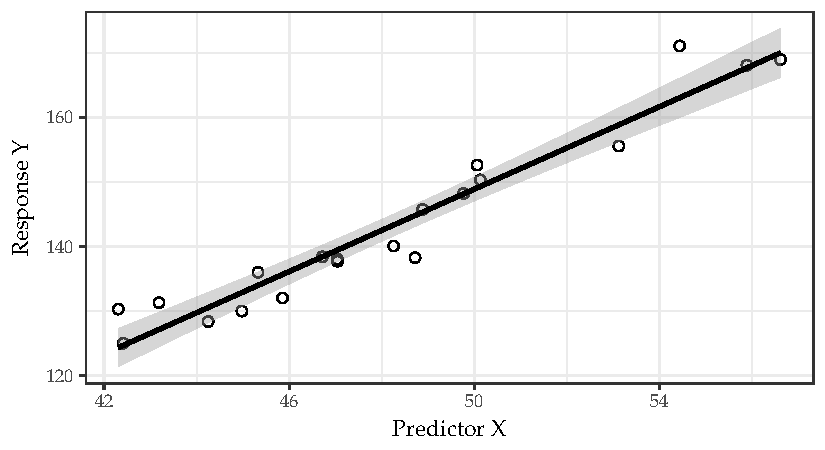
\includegraphics[width=0.9\textwidth]{./images/ci-example}
% 	\caption{\SI{95}{\percent} confidence interval for a simulated linear model $Y = - 10 + 3 X + \epsilon$, with $\sigma^{2} = 5$}
% 	\label{fig:conf-intervals}
% \end{figure}

%-----------------------------------------------------------------
\subsection{Accuracy of the model: \texorpdfstring{$R^{2}$}{R-squared} and correlation}
The goodness of a fit can be assessed by measuring the \emph{correlation coefficient} $r$, or in the more general context of \emph{multiple linear regression}, the $R^{2}$ statistic. In this section we will introduce the mathematical expressions of both coefficients and show their equivalence when studying the simple linear regression:
\begin{align}\label{eq:R2-r2}
	R^{2} = r^{2}.
\end{align}

\subsubsection{\texorpdfstring{$R^{2}$}{R-squared} statistic}
The statistic $R^{2}$ is used in the context of multiple linear regression, and particularly the simple linear regression, and is called the \emph{squared multiple correlation coefficient}, or simply \emph{R-squared}.

\bigskip
The $R^{2}$ statistic is given by
\begin{align}
	R^{2} %= \frac{\text{ESS}}{\text{TSS}}
	 	  = \frac{\text{TSS} - \text{RSS}}{\text{TSS}}
		  = 1 - \frac{\text{RSS}}{\text{TSS}}
	\qc 0 \leq R^{2} \leq 1,
\end{align}
where TSS is the \emph{total sum of squares}:
\begin{align}
	\text{TSS} = \sum_{i=1}^{n} \qty(y_{i} - \bar{y}_{i})^{2}.
\end{align}

TSS measures the total variance in the response $Y$, and can be thought of as the amount of variability inherent in the response before the regression is performed. In contrast, RSS measures the amount of variability that is left unexplained after performing the regression. Hence, $\text{TSS} - \text{RSS}$ measures the amount of variability in the response that is \emph{explained} by the regression model:
\begin{align}
	\text{ESS} = \text{TSS} - \text{RSS} = \sum_{i=1}^{n} \qty(\hat{y}_{i} - \bar{y}_{i})^{2},
\end{align}
and $R^{2}$ measures the proportion of variability in $Y$ that can be explained using $X$ as the predictor.

An $R^{2}$ statistic that is close to 1 indicates that a large proportion of the variability in the response has been explained by the regression model. A number near 0 indicates that the regression did not explain much of the variability in the response; this might occur because the linear model is wrong, the inherent error $\sigma^{2}$ is high, or both.

\subsubsection{Correlation coefficient}
A correlation coefficient is a symmetric, scale-invariant measure of association between two random variables, $X$ and $Y$. It ranges from $-1$ to $+1$, where the extremes indicate perfect correlation and 0 means no correlation. The sign is negative when large values of one variable are associated with small values of the other and positive if both variables tend to be large or small simultaneously. The most common correlation coefficient is the Pearson correlation.

\bigskip
The Pearson correlation, or Pearson's $r$, is rooted in the bivariate normal distribution $f(X, Y)$ (described in \cref{sec:bvln-distribution})
% \todo{Keep reference?}
where the theoretical correlation describes the contour ellipses for the density function. If both variables are scaled to have a variance of 1, then a correlation of zero corresponds to circular contours, whereas the ellipses become narrower and finally collapse into a line segment as the correlation approaches $\pm 1$, which is why sometimes $r$ is called the \emph{linear correlation}.

\bigskip
The empirical correlation coefficient is given by
\begin{align}
	r = \operatorname{Cor}(X,Y)
	  = \frac{\operatorname{Cov}(X,Y)}{\sqrt{\operatorname{Var}(X) \operatorname{Var}(Y) }}
	  =\frac{ \sum_{i=1}^{n} \qty(x_{i} - \bar{x}) \qty(y_{i} - \bar{y}) }{ \sqrt{\sum_{i=1}^{n} \qty(x_{i} - \bar{x})^{2} \sum_{i=1}^{n} \qty(y_{i} - \bar{y})^{2} } }
	  % \qc
	  ,\,\,\,
	  -1 \le r \le 1.
\end{align}

It can be shown that in the context of simple linear regression, the square of the correlation coefficient $r^{2}$ and the $R^{2}$ statistic are identical:
\begin{sproof}
\begin{flalign*}
	R^{2} &= 1 - \frac{\text{RSS}}{\text{TSS}}
		  = 1 - \frac{\sum_{i=1}^{n} \qty(y_{i} - \hat{y}_{i})^{2}}{\sum_{i=1}^{n} \qty(y_{i} - \bar{y}_{i})^{2}}
		  = 1 - \frac{\sum_{i=1}^{n} \qty(y_{i} - \hat{y}_{i})^{2}}{\sum_{i=1}^{n} \qty(y_{i} - \bar{y}_{i})^{2}}
		  = 1 - \frac{\sum_{i=1}^{n} \qty( y_{i} - (\hat{\beta}_{0} + \hat{\beta}_{1} x_{i}) )^{2}}{\sum_{i=1}^{n} \qty(y_{i} - \bar{y}_{i})^{2}}
		  & \\
		  &
		  =1 - \frac{\sum_{i=1}^{n} \qty( y_{i} - (\bar{y} + \hat{\beta}_{1} \bar{x} + \hat{\beta}_{1} x_{i}) )^{2}}{\sum_{i=1}^{n} \qty(y_{i} - \bar{y}_{i})^{2}}
		  = 1 - \frac{\sum_{i=1}^{n} \qty( y_{i} - \bar{y} - \hat{\beta}_{1} \qty(x_{i} - \bar{x}) )^{2}}{\sum_{i=1}^{n} \qty(y_{i} - \bar{y}_{i})^{2}}
		  \\
		  &
		  = 1 - \frac{\sum_{i=1}^{n} \qty(y_{i} - \bar{y})^{2} + \hat{\beta}_{1}^{2} \sum_{i=1}^{n} \qty(x_{i} - \bar{x})^{2} - 2 \hat{\beta}_{1} \sum_{i=1}^{n} \qty(x_{i} - \bar{x}) \qty(y_{i} - \bar{y}) }{\sum_{i=1}^{n} \qty(y_{i} - \bar{y}_{i})^{2}}
		  \\
		  &
		  = \frac{2 \hat{\beta}_{1} \sum_{i=1}^{n} \qty(x_{i} - \bar{x}) \qty(y_{i} - \bar{y}) - \hat{\beta}_{1}^{2} \sum_{i=1}^{n} \qty(x_{i} - \bar{x})^{2} }{\sum_{i=1}^{n} \qty(y_{i} - \bar{y}_{i})^{2}}
		  \\
		  &
		  = \frac{ 2 \dfrac{\sum_{i=1}^{n} \qty(x_{i} - \bar{x}) \qty(y_{i} - \bar{y})}{\sum_{i=1}^{n} \qty(x_{i} - \bar{x})^{2}} \sum_{i=1}^{n} \qty(x_{i} - \bar{x}) \qty(y_{i} - \hat{y}) - \qty( \dfrac{ \sum_{i=1}^{n} \qty(x_{i} - \bar{x}) \qty(y_{i} - \bar{y})}{\sum_{i=1}^{n} \qty(x_{i} - \bar{x})^{2}} )^{2} \sum_{i=1}^{n} \qty(x_{i} - \bar{x})^{2} }{\sum_{i=1}^{n} \qty(y_{i} - \bar{y}_{i})^{2}}
		  \\
		  &
		  %%% = \frac{ 2 \qty( \sum_{i=1}^{n} \qty(x_{i} - \bar{x}) \qty(y_{i} - \bar{y}) )^{2} - \qty( \sum_{i=1}^{n} \qty(x_{i} - \bar{x}) \qty(y_{i} - \bar{y}) )^{2} }{ \sum_{i=1}^{n} \qty(x_{i} - \bar{x})^{2} \sum_{i=1}^{n} \qty(y_{i} - \bar{y})^{2} }
		  = \frac{ \qty( \sum_{i=1}^{n} \qty(x_{i} - \bar{x}) \qty(y_{i} - \bar{y}) )^{2} }{ \sum_{i=1}^{n} \qty(x_{i} - \bar{x})^{2} \sum_{i=1}^{n} \qty(y_{i} - \bar{y})^{2} }
		  = r^{2}. \tag{\ref{eq:R2-r2} bis}
\end{flalign*}
\end{sproof}

\medskip
In simple terms, although they have the same mathematical expression, conceptually $r^{2}$ (and $r$) is an indicator of the strength of the correlation between the variables $X$ and $Y$; while $R^{2}$ is an indicator of the goodness of fit, in the sense of explained variability, of the linear model that predicts the value of $Y$ as a function of $X$ as a causal relationship. Importantly, causality in this context means the direction of causality runs from $X$ to $Y$ and not the other way round.

%-----------------------------------------------------------------
% \vfill
\vspace{0.7cm}
% \subsection{Potential problems with the assumptions}\label{sec:reg-analysis-issues}
\subsection{Regression diagnostics}\label{sec:reg-analysis-issues}

If \eqref{eq:lm-model} holds with homoscedastic random errors $\epsilon_{j}$ and if those random errors are normally distributed, or if the dataset is large, then standard distributional results will be adequate for making inferences with the OLS estimates.
This assumption of homoscedasticity is of big importance in linear regression, as the standard errors, confidence intervals, and hypothesis tests associated with the linear model rely upon it being true.

For this reason, if the errors are grossly non-normal or \emph{heteroscedastic}, meaning that their variances are unequal, then those standard results may not be reliable and a \emph{resampling method} (see \Cref{sec:resampling}) may offer genuine improvement.

\bigskip
% \newpage
To test the normality, independence, and homoscedasticity of the random errors, one can check a few diagnostic plots, which could reveal unexplained patterns in the data by the fitted model. In particular, we will focus on:
\begin{itemize}
	\item Q-Q plot of the residuals.
	\item Residuals vs fitted values plot.
\end{itemize}

\medskip
Additionally, these properties or assumptions on the random errors can be individually tested using some well known statistical hypothesis tests:
\begin{itemize}
	\item Lilliefors test: normality.
	\item Correlation test: independence.
	\item Breusch--Pagan test: homocedasticity.
\end{itemize}

\subsubsection{Q-Q plots}\label{sec:diag-qqplot}
The \emph{Q-Q plot}, or quantile-quantile plot, is a graphical tool to help us assess if a set of data plausibly came from some theoretical distribution such as a normal $\mc{N}(\mu, \, \sigma^{2})$. For example, if we run a statistical analysis that assumes our dependent variable is normally distributed, we can use a \emph{normal Q-Q plot} to check that assumption. It is just a visual check, so it is somewhat subjective, but it can help identify obvious distributional anomalies in the data.

A Q-Q plot is built by taking the sample data, sorting it in ascending order, and then plotting them versus quantiles calculated from the theoretical distribution. In the case of studying the residuals, we expect the data to follow a straight line in the normal Q-Q plot.

\subsubsection{Residuals vs fitted values plots}\label{sec:diag-resid-vs-fitted}
The \emph{residuals vs fitted values plot}, or simply residual plot, is a useful graphical tool to help us assess the homoscedasticity of the residuals or, more generally, if the residuals have non-linear patterns.

A residual plot is built by taking the residuals $\epsilon_{i}$ and plotting them versus the fitted values $\hat{y}_{i}$. The residuals should be centred on zero throughout the range of fitted values, and should be more or less uniformly distributed and have a constant spread throughout the range. The reason behind this is that
\begin{align}
	\operatorname{Cov}(\hat{y}_{i}, \epsilon_{i}) = 0.
\end{align}

One might wonder why do we not just plot the residuals $\epsilon_{i}$ vs the predictors $x_{i}$. Actually, one could plot the residuals vs the predictors, instead of vs the fitted values. However, this plot would be impossible to visualise if we had more than two predictors, so it is of standard practice to look at the residuals vs fitted plot, which is always a 2D plot.

Usually, the residual plot is accompanied by a \emph{locally weighted scatterplot smoothing} (LOWESS) line to help visualise the trend of the residuals. Naturally, under the assumption of normality, the trend should follow a horizontal line centred at $\epsilon = 0$. It is also useful to show the outer quantiles of the residuals to help emphasise and distinguish patterns.

\subsubsection{Lilliefors test}\label{sec:diag-lillie}
The \emph{Lilliefors test}, developed by \citeauthor{Lilliefors1967} (\citeyear{Lilliefors1967}) \cite{Lilliefors1967}, is  a normality test based on the Kolmogorov--Smirnov (KS) test. It is used to test the null hypothesis that data comes from a normally distributed population when the null hypothesis does not specify which normal distribution; in other words, it does not specify the expected value $\mu$ and variance $\sigma^{2}$ of the distribution.

Like most statistical tests, this test of normality defines a criterion and gives its sampling distribution (in this case, a Kolmogorov--Smirnov distribution). When the probability, or $p$-value, associated with the criterion is smaller than a given $\alpha$ significance level, the alternative hypothesis is accepted (i.e., we conclude that the sample does not come from a normal distribution).

A thing to consider with this test is that with small samples, the KS test is underpowered and fails to detect true violations of normality; and with large samples, the KS test may detect violations of normality which are not important for practical purposes~\cite{Razali2010}. For this reason it is important when assessing normality to also look at indicators of the degree of normality such as the Q-Q plot stated previously.

\medskip
In R, the \texttt{nortest} package offers the \texttt{lillie.test()} function to perform the Lilliefors test.

\subsubsection{Correlation test}\label{sec:diag-covtest}
The \emph{Correlation test} is a test based on either Pearson's product-moment correlation, Kendall's rank correlation tau, or Spearman's rank correlation rho. It is used to test the null hypothesis that the correlation between paired samples (in this case, $\epsilon$ and $\hat{Y}$) is zero.

The three methods use different measures of correlation, all in the range $[-1, 1]$ with $0$ indicating no correlation. The most used method is Pearson's product-moment correlation, in which the test statistic is based on Pearson's product moment correlation coefficient $r = \operatorname{Cor}(\epsilon, \hat{Y})$ and follows a Student's $t$-distribution on $n-2$ degrees of freedom.

\medskip
In R, the \texttt{stats} package offers the \texttt{cor.test()} function to perform the Lilliefors test.

\subsubsection{Breusch--Pagan test}\label{sec:diag-bptest}
The \emph{Breusch--Pagan test}, developed by \citeauthor{Breusch1979} (\citeyear{Breusch1979}) \cite{Breusch1979}, is a test used in regression analysis to test for homoscedasticity. It is used to test the null hypothesis that residuals are homoscedastic.

The null hypothesis is that the residual variances are all equal, while the alternative hypothesis is that the residual variances are a multiplicative function of one or more variables. To do this, the test fits a linear regression model to the residuals of a linear regression model (by default the same explanatory variables are taken as in the main regression model) and rejects if too much of the variance is explained by the additional constructed explanatory variables.

\medskip
In R, the \texttt{lmtest} package offers the \texttt{bptest()} function to perform the Breusch--Pagan test.

% \subsubsection{Goldfeld--Quandt test}
% The \emph{Goldfeld--Quandt test} is a test used in regression analysis to test for homoscedasticity. It compares variances of two subgroups; one set of high values and one set of low values. If the variances $\sigma^{2}_{1}$ and $\sigma^{2}_{2}$ differ, the test rejects the null hypothesis that the variances of the errors are not constant.

% Although Goldfeld and Quandt described two types of test in their paper (parametric and non-parametric), the term \emph{Quandt Goldfeld test} usually means the parametric test. The assumption for the test is that the data is normally distributed.

% \medskip
% In R, the \texttt{lmtest} package offers the \texttt{gqtest()} function to perform the Goldfeld-–Quandt test.

\bigskip
\begin{example}
	Let us consider the three different simulated models depicted in \Cref{fig:models-example}. For each of the models, the random error has been built under a different assumption: (a) homoscedasticity, (b) heteroscedasticity, and (c) non-normality.

	For a moment let us forget we know the models behind the data and let us see what we can infer purely from the data, which is generally the case when dealing with real data.

	\begin{figure}[H]
		\centering
		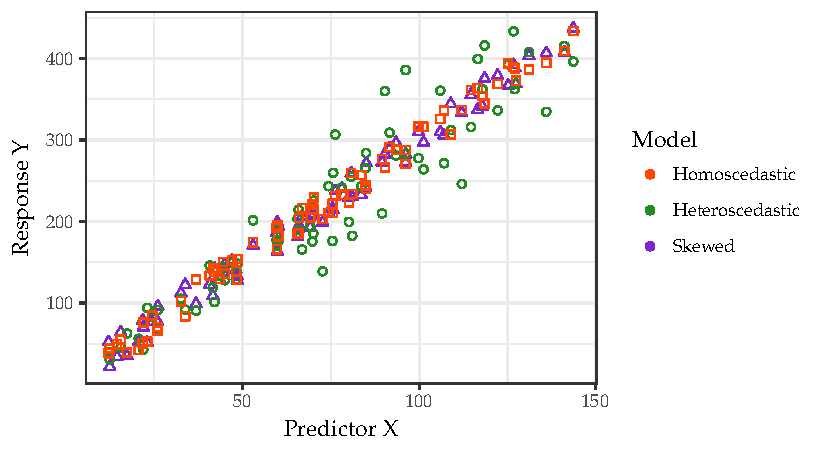
\includegraphics[width=0.8\textwidth]{./images/models-example}
		\caption{Three simulated models of 75 observations each with different response $Y$ in which it would seem appropriate to fit a linear model using OLS}
		\label{fig:models-example}
	\end{figure}

	Looking at the Q-Q plots, at first glance it seems that both \Cref{fig:qq-example-a} and \Cref{fig:qq-example-b} follow a normal distribution for the residuals. A priori, what we can say is that the tails in \Cref{fig:qq-example-a} are slightly lighter than what we would expect under the standard modelling assumptions, while the tails in \Cref{fig:qq-example-b} are heavier.

	As a contrast, the Q-Q plot gives \Cref{fig:qq-example-a} immediately tells us that we are under a clear case of non-normality and that the fitted model should be probably reconsidered.
	\begin{figure}[H]
		\centering
		\subfloat[Homoscedastic model]{%
			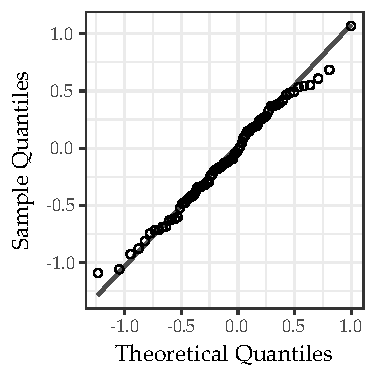
\includegraphics[width=0.32\textwidth]{./images/qq-norm-example}
			\label{fig:qq-example-a}%
			}%
		\subfloat[Heteroscedastic model]{%
			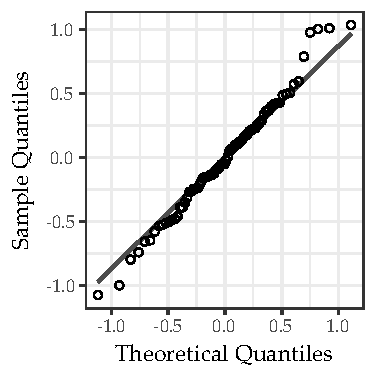
\includegraphics[width=0.32\textwidth]{./images/qq-hetero-example}
			\label{fig:qq-example-b}%
			}%
		\subfloat[Skewed model]{%
			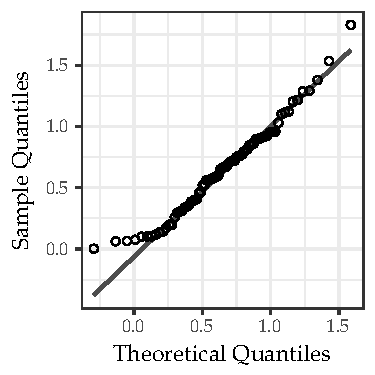
\includegraphics[width=0.32\textwidth]{./images/qq-skewed-example}
			\label{fig:qq-example-c}%
			}%
		\caption{Normal Q-Q plots for the three models simulated in \Cref{fig:models-example}}
		\label{fig:qq-example}
	\end{figure}

	Let us see if a residual plot can provide additional insight to the underlying models depicted in \Cref{fig:models-example} that could not be observed in the Q-Q plots in \Cref{fig:qq-example}.
	\begin{figure}[H]
		\centering
		\subfloat[Homoscedastic model]{%
			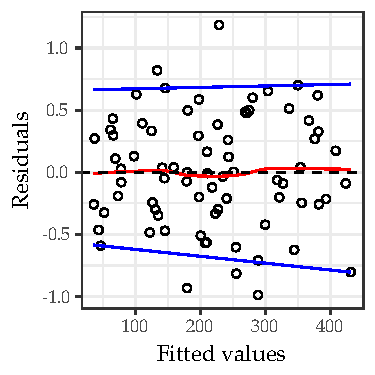
\includegraphics[width=0.32\textwidth]{./images/resid-norm-example}
			\label{fig:resid-example-a}%
			}%
		\subfloat[Heteroscedastic model]{%
			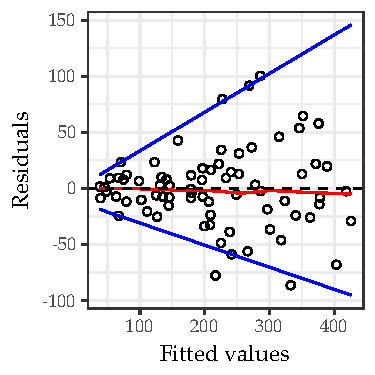
\includegraphics[width=0.32\textwidth]{./images/resid-hetero-example}
			\label{fig:resid-example-b}%
			}%
		\subfloat[Skewed model]{%
			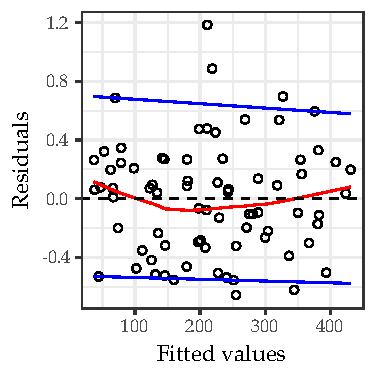
\includegraphics[width=0.32\textwidth]{./images/resid-skewed-example}
			\label{fig:resid-example-c}%
			}%
		\caption[Residual plots for the three models simulated in \Cref{fig:models-example}]{Residual plots for the three models simulated in \Cref{fig:models-example}, the red line is a smooth fit to the residuals, and the blue lines are the outer quantiles of the residuals}
		\label{fig:resid-example}
	\end{figure}

	In \Cref{fig:resid-example-a} and \Cref{fig:resid-example-c} we can see that the residuals appear to be roughly randomly distributed. However, for \Cref{fig:resid-example-c}, it is clear that the residuals are skewed, as the point pattern is densest somewhere other than the centre line; this tells us that the residuals do not follow a normal distribution at all. But we already knew this from \Cref{fig:qq-example-c}.

	In \Cref{fig:resid-example-b} we can see quite an extreme case of heteroscedasticity, as the magnitude of the residuals tends to increase with the fitted values, giving place to a prominent funnel shape. This tells us that there is some kind of correlation between the residuals and the predictors: $\epsilon_{i} \sim \hat{y}_{i} = f(x_{i})$.
	% \begin{figure}[H]
	% 	\centering
	% 	\subfloat[Homoscedastic model]{%
	% 		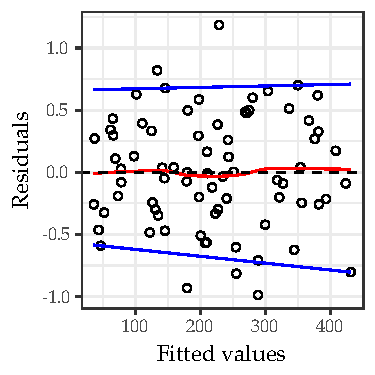
\includegraphics[width=0.32\textwidth]{./images/resid-norm-example}
	% 		\label{fig:resid-example-a}%
	% 		}%
	% 	\subfloat[Heteroscedastic model]{%
	% 		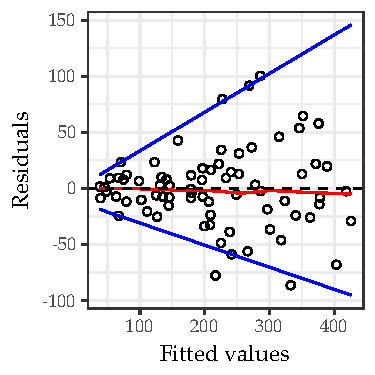
\includegraphics[width=0.32\textwidth]{./images/resid-hetero-example}
	% 		\label{fig:resid-example-b}%
	% 		}%
	% 	\subfloat[Skewed model]{%
	% 		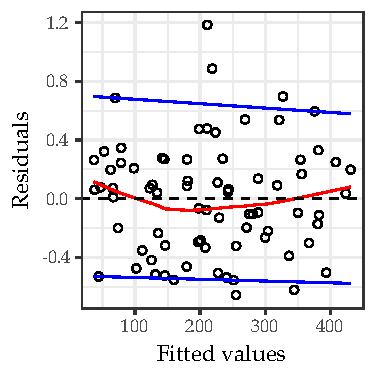
\includegraphics[width=0.32\textwidth]{./images/resid-skewed-example}
	% 		\label{fig:resid-example-c}%
	% 		}%
	% 	\caption{Residual plots for the three models simulated in \Cref{fig:models-example}, the red line is a smooth fit to the residuals, and the blue lines are the outer quantiles of the residuals}
	% 	\label{fig:resid-example}
	% \end{figure}

	As a last step, let us explore the results of performing the Lilliefors, correlation, and Breusch--Pagan tests in \Cref{tab:stat-tests-example}.
	\begin{table}[H]
		\centering
		\begin{tabular}{lccc}
			\toprule
			\toprule
			Model           & Lilliefors  & Correlation & Breusch--Pagan \\
			\midrule
			(a) Homoscedastic   & \num{0.649} & \num{1.000} & \num{0.312} \\
			(b) Heteroscedastic & \num{0.054} & \num{1.000} & \num{0.004} \\
			(c) Skewed          & \num{0.723} & \num{1.000} & \num{0.830} \\
			\bottomrule
		\end{tabular}
		\caption{List of $p$-values associated with the statistical hypothesis tests to respectively analyse normality, independence, and homoscedasticity of the residuals on the three simulated models}
		\label{tab:stat-tests-example}
	\end{table}

	From the results in \Cref{tab:stat-tests-example} we can see that the Lilliefors fails to reject the non-normality of the heteroscedastic and skewed models, when in fact only the homoscedastic model is simulated following a normal distribution, and that there is no correlation between the residuals and the fitted values for any of the models. More importantly, though, the Breusch--Pagan test successfully rejects homoscedasticity in the grossly heteroscedastic model.
\end{example}

%-----------------------------------------------------------------
\bigskip
To sum up, for linear regression with normal random errors having constant variance, the OLS theory of regression estimation provides clean, exact methods for analysis. But for generalisations to non-normal errors and non-constant variance, exact methods rarely exist, and we are faced with approximate methods based on linear approximations to estimators and central limit theorems. In the next section we will explore how resampling methods have the potential to provide a more accurate analysis.
